% !TEX root = cikm2018-visual-ltr.tex

\section{Method}
In this section we proposing a multimodal architecture used to train a \ac{LTR} model with both visual and content features. 
The first two paragraphs describe the implementation of three visual feature extractors, being:
\begin{inparaenum}[(i)]
\item the VGG-16~\cite{simonyan2014very} classification model pretrained on ImageNet, and
\item the ResNet-152~\cite{he2016deep} classification model pretrained on ImageNet.
\end{inparaenum} 
In the last paragraph, we propose the use of a saliency model to create synthetic saliency heatmaps for each of the input images. These synthetic saliency images are trained to learn a more expressive representation of the viewing pattern of a user. 

All corresponding code is available on Github.\footnote{URL removed for review}

\subsection{Multimodal Architecture}
In order to compare the performance of various visual feature extractor methods, we propose a reusable multimodal architecture. 
The multimodal architecture is visualized in Figure~\ref{fig:multimodelarchitecture}. 
The model starts by taking an image $x_{v}$ (1) as an input to the visual feature extraction layer (2) in order to create a generic visual feature vector $x_{vf}$. In turn, $x_{vf}$ is then used as an input to the visual feature transformation layer (3).
This visual feature transformation layer learns to transforms the generic visual features to a \ac{LTR} specific visual feature vector $x_{vl}$.

The final \ac{LTR} feature vector $x_{l}$ is constructed by concatenting the visual \ac{LTR} features $x_{vl}$ with the content \ac{LTR} features $x_{c}$ (4). 

$x_{l}$ is then used as an input to the scoring component (5), which transforms the features to a single score for each document-query pair. The scoring component uses a single fully connected layer with a hidden size of $10$ and dropout empirically set to $10\%$. The resulting model is trained end-to-end using a pairwise hinge loss with $L_2$ regularization. 

% \begin{multline}
% x_{vl} = f_{t}(f_{v}(x_{v})) \\ x_{s} = f_{s}(x_{vl} \oplus x_{c}) 
% \end{multline}


\begin{figure}[t]
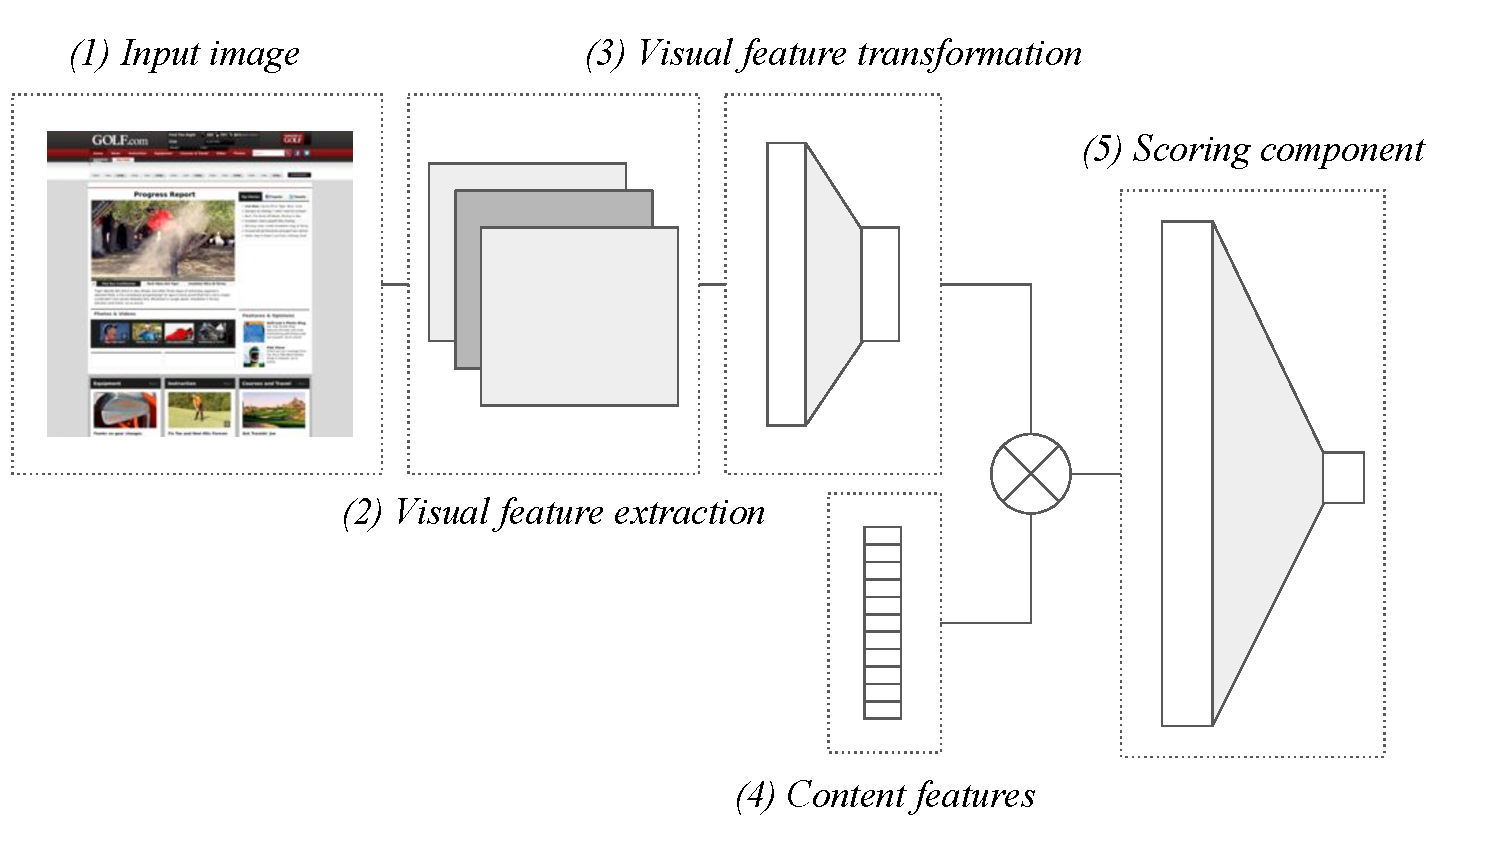
\includegraphics[width = 3.5in]{images/multimodelarchitecture.pdf}
\caption{The proposed multimodal architecture, which the visual feature extraction}
\label{fig:multimodelarchitecture}
\end{figure}

\subsection{Visual Feature Extractors}
Since the \datasetname{} data\-set that we introduce in this paper has a relatively low number of snapshots to train a separate feature extractor, we use the VGG-16~\cite{simonyan2014very} and ResNet-152~\cite{he2016deep} models from Torchvision,\footnote{\url{https://pytorch.org/docs/stable/torchvision/models.html}} pretrained on ImageNet, as two separate feature extractors. 
\paragraph{VGG-16}
VGG-16 is commonly used in literature for training transfer-learned models. 
Although VGG-16 is not the current state-of-the-art visual feature extractor, it is a reasonable trade-off between effectiveness and simplicity.
The VGG-16 architecture consists of a set of convolutional filters and fully connected layers. 
The convolutional filters extract features from the input image, which are used by the fully connected layers to classify the image. 
These filters are generic with respect to input and task~\citep{donahue2014decaf}, which make them suitable for being used as a visual feature extractor to create generic visual features $x_{vf}$. We use the convolutional layers as is, by freezing all the parameters during training. The fully connected layers can be altered and retrained in order to be used with new inputs and tasks, making them suitable to be used as a visual feature transformation layer. We replace the last fully connected layer by a newly initialized fully connected layer in order to produce $x_{vl}$. The size of $x_{vl}$ was set to $30$ which was empirically found to provide good performance in preliminary results. Both the parameters of the retained and new fully connected layers are further optimized during training.

\paragraph{ResNet-152}
The ResNet-152~\cite{he2016deep} architecture has a significant increase in ImageNet classification performance over VGG-16. The residual connections between convolutional layers allow for deeper networks to be trained without suffering from vanishing gradients. The original ResNet-152 architecture only has a single fully connected layer, which empirically showed to not be enough to successfully train the model. Instead, we train a fully connected network from scratch. The network was constructed using three layers with $4096$ hidden units and a final layer resulting in $x_{img\_ltr}$ with a size of $30$, which was empirically found to provide good performance in preliminary results.

\subsection{Saliency Heatmaps}
In order to increase the ability to learn the visual quality of a webpage, we propose to explicitly model the user viewing pattern by using synthetic saliency heatmaps. 
Following \cite{shan2017two}, we implemented and trained a two-stage transfer learning model that learns how to predict saliency heatmaps on web pages.
Similarly to the visual feature extraction approaches in the paragraphs above, \cite{shan2017two} takes a pretrained image recognition model and finetunes the output layers on the following two datasets in order respectively:
\begin{inparaenum}[(i)]
\item SALICON by \cite{jiang2015salicon}, a large dataset containing saliency heatmaps created with eye-tracking hardware on natural images, and 
\item the webpage saliency dataset by \cite{shen2014webpage}, a smaller dataset containing saliency heatmaps created with eye-tracking hardware on web pages.
\end{inparaenum}

The trained model is applied to the $3\times224\times224$ input images from the \datasetname~data\-set, resulting in grayscale heatmaps with a dimension of $1\times64\times64$. These heatmaps can then be used as the $x_{v}$ for the visual feature extractors described above by linearly scaling them to $3\times224\times224$, matching them with the VGG-16 and ResNet-152 input dimensions. Figure~\ref{fig:exampleshots} shows example snapshots with their corresponding saliency heatmaps.

The saliency heatmaps generated using this method have various advantages over the usage of vanilla and keyword highlighted snapshots because synthetic saliency heatmaps
\begin{inparaenum}[(i)]
\item explicitly learn to predict the viewing pattern by training an end-to-end model on actual eye-tracking data, and 
\item reduce the average storage requirement by $93.5\%$ and $77\%$ respectively compared to the $3\times224\times224$ snapshot images when stored as $1\times64\times64$ and $3\times224\times224$ saliency heatmap images.
\end{inparaenum}
